\documentclass{beamer}
%\documentclass[trans]{beamer}
%\documentclass[handout]{beamer}

\mode<presentation>
{
	%\usetheme{Malmoe}
	\usetheme[secheader]{Boadilla}
	\setbeamercovered{transparent}
}

\usepackage[english]{babel}
\usepackage[latin1]{inputenc}

\usepackage{times}
\usepackage[T1]{fontenc}
% Or whatever. Note that the encoding and the font should match. If T1
% does not look nice, try deleting the line with the fontenc.

\usepackage{graphicx,pgf,tikz}
\usepackage{multicol}
\usetikzlibrary{fadings}
\usepackage[]{algorithm2e}
\usepackage{subfig}
\usepackage{tabularx}
\usepackage{multirow}
 \usepackage{setspace}
 \usepackage{CJK}
 
 \newlength{\alignheight}
 \newlength{\alignwidth}
 \newcommand{\fakeheight}[3]{%
   \makebox[#1][c]{\rule[-.5\dimexpr#2\relax]{0pt}{#2}\raisebox{-.5\height}{#3}}%
 }

%\usepackage{latexsym}
%\renewcommand{\baselinestretch}{1.2}

\newcommand{\real}{I\!\!\!R}
\newcommand{\bin}{I\!\!\!B}
%\newcommand{\cA}{{\mathcal{A}}}
%\newcommand{\bA}{\bar{\mathcal{A}}}
\newcommand{\cA}{\mathcal{A}}
\newcommand{\bA}{\bar{A}}
\newcommand{\my}{\Gamma} %{M(\bar{y})}
\newcommand{\lb}{\nu}
\newcommand{\scaleAA}{\omega}
\newcommand{\scalei}{\eta_i}
\newcommand{\recipscalep}{\frac{1}{\eta_p}}

\newcommand{\cG}{\mathcal{G}}

\newcommand{\wt}{\widetilde}
\newcommand{\wto}{\widetilde\omega}
\newcommand{\wh}{\widehat}

\newcommand{\sgn}{{\rm sgn}}
\newcommand{\epc}{\hspace{1pc}}
\newcommand{\diag}{{\rm diag}}
\newcommand{\sol}{{\rm SOL}}
\newcommand{\onebld}{{\mbox{\boldmath $1$}}}
\newcommand{\twobld}{{\mbox{\boldmath $2$}}}
\newcommand{\Abld}{{\mbox{\boldmath $A$}}}
\newcommand{\xbld}{{\mbox{\boldmath $x$}}}
\newcommand{\ubld}{{\mbox{\boldmath $u$}}}
\newcommand{\thalf}{{\textstyle \frac{1}{2}}}
\newcommand{\zbld}{{\mbox{\boldmath $z$}}}
\newcommand{\Bbld}{{\mbox{\boldmath $B$}}}
\newcommand{\Cbld}{{\mbox{\boldmath $C$}}}
\newcommand{\Dbld}{{\mbox{\boldmath $D$}}}
\newcommand{\bigf}{\mathcal{F}}
\newcommand{\bigt}{\mathcal{T}}
\newcommand{\bign}{\mathcal{N}}
\newcommand{\SCGF}{\scriptstyle {\mathrm GF}}
\newcommand{\SCNP}{\scriptstyle {\mathrm NP}}

%\newcommand{\ds}{{\textcolor{red}{\circle*{10}}}}
%\newcommand{\tri}{{\textcolor{blue}{\circle*{10}}}}
%\newcommand{\cs}{{\textcolor{green}{\circle*{10}}}}
%\newcommand{\sps}{{\textcolor{yellow}{\circle*{10}}}}

\newcommand{\bz}{\bar{z}}
\newcommand{\tx}{\tilde{x}}
\newcommand{\ty}{\tilde{y}}
\newcommand{\half}{\frac{1}{2}}

\newcommand{\scwork}{\mbox{\scriptsize work}}
\newcommand{\sclb}{\mbox{\scriptsize lb}}
\newcommand{\scub}{\mbox{\scriptsize ub}}

\definecolor{orange}{rgb}{1,0.5,0}
\newcommand{\torange}{\textcolor{orange}}

\newcommand{\tred}{\textcolor{red}}
\newcommand{\tblue}{\textcolor{blue}}
\newcommand{\tmag}{\textcolor{magenta}}
\newcommand{\tgreen}{\textcolor{green}}
\newcommand{\tcyan}{\textcolor{cyan}}
\newcommand{\bbb}{\textcolor{blue}}
\newcommand{\grr}{\textcolor{purple}}
\newcommand{\tgrey}{\textcolor{gray!25}}
\newcommand{\tpink}{\textcolor{red!60}}
\newcommand{\tcam}{\textcolor{blue!40}}

%\newcommand{\ds}{\textcolor{red}{\circle*{10}}}
%\newcommand{\tri}{{\textcolor{blue}{\circle*{10}}}}
%\newcommand{\cs}{{\textcolor{green}{\circle*{10}}}}
%\newcommand{\sps}{{\textcolor{yellow}{\circle*{10}}}}

%\textheight 8.8in

%\pagestyle{myheadings}


%\markboth{Draft of \today}{Draft of \today}

\newcommand{\til}{\char '176}
\newcommand{\ds}{{\textcolor{red}{\circle*{10}}}}
\newcommand{\tri}{{\textcolor{blue}{\circle*{10}}}}
\newcommand{\cs}{{\textcolor{green}{\circle*{10}}}}
\newcommand{\sps}{{\textcolor{yellow}{\circle*{10}}}}
\newcommand{\tr}{\mbox{trace}}
\newcommand{\re}{I\!\!\!R}
\def\R{{\re}}

%\newtheorem{theorem}{Theorem}
%\newtheorem{lemma}{Lemma}
\newtheorem{proposition}{Proposition}
%\newtheorem{corollary}{Corollary}
%\newtheorem{definition}{Definition}
%\newtheorem{hypothesis}{Hypothesis}

% Definition of the proof-environment:
%\newenvironment{proof}{{\raggedright\bf Proof:}\quad}{\hspace*{\fill}$\fbox{ }$\\}

% Delete this, if you do not want the table of contents to pop up at
% the beginning of each subsection:
%\AtBeginSubsection[]
%{
%  \begin{frame}<beamer>
%    \frametitle{Outline}
%    \tableofcontents[currentsection,currentsubsection]
%  \end{frame}
%}
\AtBeginSection[]
{
	\begin{frame}<beamer>
		\frametitle{Outline}
		\tableofcontents[currentsection,currentsubsection]
	\end{frame}
}

% If you wish to uncover everything in a step-wise fashion, uncomment
% the following command: 

\beamerdefaultoverlayspecification{<+->}

\title[Robust Scheduling]{A Robust Approach for Project Scheduling Problem}
\author[Shen, Yang]{Xin Shen, Jubiao Yang\\{\small advised by: John E. Mitchell}}

\institute[RPI]{ 
Rensselaer Polytechnic Institute  \\
Troy,  NY  12180}

\date[MOPTA 2015]{7th AIMMS-MOPTA Optimization Modeling Competition\\\textit{Lehigh University, Bethlehem, PA}, 2015}

\begin{document}
	\bibliographystyle{plain}

	\begin{frame}
		\titlepage
	\end{frame}
%\nocite{basescu2,JEM_selorth,basescu3}

	\section*{Outline} 
		\begin{frame}[allowframebreaks]
			\tableofcontents 
		\end{frame}

	\section{Introduction}
		\begin{frame}
			\frametitle{Introduction}
			\textbf{Objective}: to maximize the net present value of the project portfolio (sum of benefits and costs of portfolio projects discounted appropriately with hurdle rate).\\
			\bigskip
			Projects may have \textit{dependencies}:\\
			\smallskip
			$\bullet$ \tmag{nonsimultaneity} (e.g. resource constraints on teams/equipments)\\
			\smallskip
			$\bullet$ \tcam{single precedence} (e.g. a project is decomposed into phases)\\
			\smallskip
			$\bullet$ \tgreen{alternative precedence} (e.g. parallel-approach effort to overcome a technical hurdle)
		\end{frame}
		
		\begin{frame}
			\frametitle{Introduction}
			Projects are subject to risks of bad luck (\torange{delay}/\tred{failure}/\tcyan{delay and failure}).\\
			\bigskip
			\textbf{\textit{Deterministic Approach}}: prepare for a certain bad-luck scenario beforehand (incl. scenario with no bad luck) and schedule a portfolio.\\
			\smallskip
			disproportionate depreciation of portfolio value can be caused by "chain reaction" of bad lucks, thanks to project dependencies.\\
			\bigskip
			\textbf{\textit{Robust Approach}}: to have the largest portfolio value under the worst possible outcome scenario (resilience to bad luck).
		\end{frame}

	\section{Deterministic Approach}
		\begin{frame}
			\frametitle{Project dependencies}
			%Dependencies can be modeled with a single matrix $\Delta_{ij}$:\\
			%\smallskip
			\tmag{nonsimultaneity}: if $i \nsim j$, then $\Delta_{ij}=\Delta_{ji}=-1$\\
			\smallskip
			\tgreen{alternative precedence}: if $\{i_1,\cdots,i_N\} \vdash j$, then $\Delta_{i_{1}j}=\cdots=\Delta_{i_{N}j}=\text{a unique positive integer}$\\
			\smallskip
			\tcam{single precedence}: $i \succ j~~\Leftrightarrow~~\{i\} \vdash j$, thus a special case of $I \vdash j$ and can be treated the same way\\
			\medskip
			e.g. for a project pool of $\{p_1,p_2,p_3,p_4,p_5\}$ with $p_1 \nsim p_2$, $p_2 \nsim p_3$, $p_3 \succ p_1$, $p_1 \succ p_4$, $\{p_2,p_5\} \vdash p_4$, $p_3 \succ p_4$, $\{p_1,p_3\} \vdash p_5$:\\
			\smallskip
			\begin{equation*}
				\boldsymbol{\Delta}=
				\bordermatrix{     & p_1 & p_2 & p_3 & p_4 & p_5\cr
				   p_1 &     &  -1 &     &  1  &  1 \cr
				   p_2 &  -1 &     & -1  &  2  &    \cr
				   p_3 &  1  & -1  &     &  3  &  1 \cr
				   p_4 &     &     &     &     &    \cr
				   p_5 &     &     &     &  2  &    }
			\end{equation*}
		\end{frame}

		\begin{frame}
			\frametitle{Model}
			Binary variable $X_{jt}$:
			\begin{equation*}
				X_{jt}=
				\begin{cases}
					1, & \text{if Project } j \text{ starts at the beginning of the } i^{th} \text{ month} \\
					0, & \text{otherwise}
				\end{cases}
			\end{equation*}
			User-controlled binary parameters $q^{\delta}_j$ and $q^f_j$:
			\begin{equation*}
				\begin{array}{cl}
					q^{\delta}_j= &
					\begin{cases}
						1, & \text{if knew beforehand that Project } j \text{ would be delayed} \\
						0, & \text{otherwise}
					\end{cases}\\
					q^{f}_j= &
					\begin{cases}
						1, & \text{if knew beforehand that Project } j \text{ would fail} \\
						0, & \text{otherwise}
					\end{cases}\\
				\end{array}
			\end{equation*}
			Thus the adjusted durations and costs are:
			\begin{equation*}
				\tilde{d}_j=d_j+q^{\delta}_j d^+_j
				,~
				\tilde{c}_j=c_j+q^{\delta}_j c^+_j
				,~\forall j \in J
			\end{equation*}
		\end{frame}
		
		\begin{frame}
			\frametitle{Formulation}
			\begin{itemize}
				\item a project can start at most once:
					\begin{equation*}
						\sum\limits_{t=1}^{T} X_{jt} \leq 1-q^f_i,~\forall j \in J
					\end{equation*}
				\item a project cannot start if it cannot complete by the deadline:
					\begin{equation*}
						\sum\limits_{t\geq T+1-\tilde{d}_j} X_{jt}=0,~\forall j \in J
					\end{equation*}
				\item for $i \nsim j$, i cannot be started within $d_j$ months after j started, vice versa:
					\begin{equation*}
						\sum\limits_{t-\tilde{d}_j+1\leq t'\leq t+\tilde{d}_i-1} X_{jt'} + X_{it} \leq 1,~\forall i \nsim j,~\forall t \in \{1,\cdots,T\}
					\end{equation*}
			\end{itemize}
		\end{frame}
		
		\begin{frame}
			\frametitle{Formulation}
			\begin{itemize}
				\item for $I\,\vdash\,j$, j cannot be started until at least one of the projects in I has been finished:
					\begin{equation*}
						\label{EqnAnyPrecedence}
						\sum\limits_{i\in I}\sum\limits_{t'\leq t-\tilde{d}_i} X_{it'} \geq X_{jt},~\forall I \vdash j,~\forall t \in \{1,\cdots,T\}
					\end{equation*}
				\item the objective function can be evaluated:
					\begin{equation*}
						NPV_{\gamma}(S,T) = -\sum\limits_{j,t} \gamma^t \cdot \tilde{c}_j \cdot X_{jt} + \sum\limits_{j,t} \gamma^{t+\tilde{d}_j} \cdot b_j \cdot X_{jt}
					\end{equation*}
			\end{itemize}
		\end{frame}



\section{Robust Scheduling}
\begin{frame}
\frametitle{Problem Description}
Define:\\
\begin{align*}
	&I_f\,=\, \{\mbox{Project that fails}\}\\
	&I_{\delta}\,=\, \{\mbox{Project that delays but succeeds}\}\\
	&I_{f|\delta}\,=\, \{\mbox{Project that delays and then fails}\}\\
\end{align*}
Each project has probabilities to delay, to fail, or to delay and then fail. The cost of each occurence of bad luck can be calculated from these probabilities. The total cost must be less than or equal to the bad luck budget.\\
%\begin{equation*}
%	w(I_f, I_{\delta}, I_{f|\delta})\,:=\,\sum_{j\in I_f} [-log_2(p_{f,j})]\,+\,\sum_{j\in I_{\delta}}[-log_2((1-p_{f,j})p_{\delta,j})]\,+\,\sum_{j\in I_{f|\delta}}[-log_2((1-p_{f,j}))]
%\end{equation*}
\medskip
\tblue{Given a bad luck budget W,  want to find a schedule $(S, T)$ that yields the largest NPV in the worst case.}
\end{frame}

%\begin{frame}
%\frametitle{General Framework}
%\\
%\bigskip
%The decision maker can update the schedule when any bad luck happens. The process is called \tblue{Adaptive Scheduling}.\\
%\bigskip
%We use a '\tblue{Solve-Robustify}' approach to find a robust schedule under Adaptive Scheduling.
%\end{frame}


\begin{frame}
\frametitle{Adaptive Scheduling}
\tmag{The schedule will be updated once any bad luck happens.}
% insert a figure
The purpose is to reduce the loss. \\
\bigskip
Assumptions:
\begin{itemize}
%\item Only projects selected in the original schedule can be chosen in the updated schedule.
%\medskip
\item Bad Luck only happens to a project at its scheduled ending time.
\medskip
\item Only projects that are scheduled to start at and after the time of bad luck can be updated.
\medskip
\item When updating the schedule, we don't take future bad luck into account.
\end{itemize}
\end{frame}

\begin{frame}
\frametitle{Adaptive Scheduling}
Example:
\begin{displaymath}
\begin{array}{ll}
&1\succ 2\succ 3~\mbox{and}~c_1=c_2=c_3=1\\
&b_1=b_2=0, b_3=10, d_1=d_2=d_3=12
\end{array}
\end{displaymath}
The deadline is Month 36
\begin{figure}
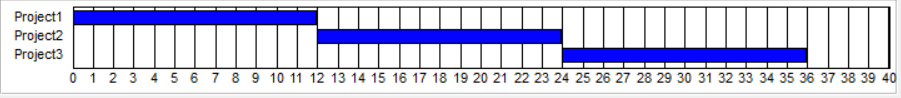
\includegraphics[scale=0.35, width=11cm, height=2.5cm]{Adapt1.png}
\caption{Initial Schedule}
\end{figure}
\end{frame}



\begin{frame}
\frametitle{Adaptive Scheduling}
\begin{figure}
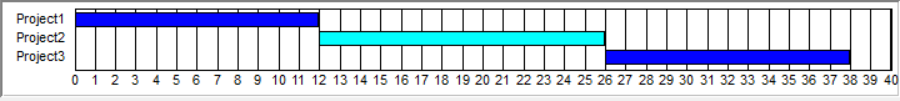
\includegraphics[scale=0.35, width=11cm, height=1.5cm]{Adapt2.png}
\caption{Project 2 delayed by 2 months}
\end{figure}
Project 3 cannot be completed by the deadline.
\begin{figure}
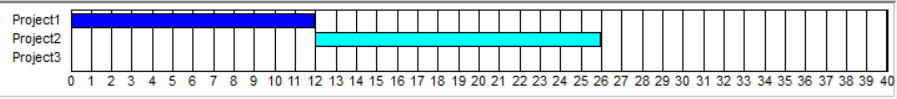
\includegraphics[scale=0.35, width=11cm, height=1.5cm]{Adapt3.png}
\caption{Updated Schedule after Delay}
\end{figure}
Delete Project 3 in the updated schedule.
\end{frame}

\begin{frame}
\frametitle{Adaptive Scheduling}
\bigskip
Given an initial schedule $\tblue{(S, T)}$ and a triple of bad luck $\tblue{(I_f, I_{\delta}, I_{f|\delta})}$, can simulate and get a final realization $\tblue{(S', T')}$ by solving a series of optimization problems.
\end{frame}



\begin{frame}
\frametitle{General Framework}
We use a \tblue{Solve and Robustify} approach to find a robust schedule.
\medskip
\begin{algorithm}[H]
         \KwData{Initial Schedule $(S,T)$, budget of bad luck W}

%	\KwResult{Robust Schedule $(S', T')$}.

	\While{Stopping Criteria not satisfied}{

		Find $(I_f, I_{\delta}, I_{f|\delta})$ in the worst case scenario under \tblue{Adaptive Scheduling}\;

                  Robustify $(S, T)$ based upon $(I_f, I_{\delta}, I_{f|\delta})$ \;
	}       

Output $(S,T)$
\end{algorithm} 
\medskip

The initial schedule can be the solution in the simple case.
\end{frame}

\begin{frame}
\frametitle{Estimation of Worst Case Scenario}
 Given the budget W, want to find a triple of bad luck $\tblue{(I_f, I_{\delta}, I_{f|\delta})}$ that maximizes the loss.\\
\bigskip
Cannot incorporate adaptive scheduling into a single optimization problem.\\
\bigskip
\tblue{Brute-force approach}: Try every combination of $(I_f, I_{\delta}, I_{f|\delta})$ and pick the one that yields the maximum loss. Computationally infeasible.
\end{frame}

\begin{frame}
\begin{itemize}
\frametitle{Estimation of Worst Case Scenario}
%\bigskip
\item Our approach: \tblue{Greedy Heuristics}.
\bigskip
\item Pros: Computationally efficient. Can get a bad scenario and identify critical projects in a reasonable amount of time.
\bigskip
\item Cons: No proof for the optimality of $\tblue{(I_f, I_{\delta}, I_{f|\delta})}$.
\end{itemize}
\end{frame}

    \begin{frame}
\frametitle{Estimation of Worst Case Scenario}

\begin{algorithm}[H]
\KwData{Initial Schedule (S,T), budget of bad luck W,$(I_f, I_{\delta}, I_{f|\delta})=\emptyset$}
\KwResult{Triple of bad luck in the worst case $(I_f, I_{\delta}, I_{f|\delta})$}
\While{The bad luck budget is not used up}{
Add the project with type of bad luck that yields the maximum loss into the triple $(I_f, I_{\delta}, I_{f|\delta})$.
%	\For{i in S, p in $\{Failure, delay, both\}$ with $W_{ip}\leq W$}{
% 
% 
%	}
%	\eIf{There exist some project i with type bad luck that incurs positive loss}{
%	pick the one that with the largest loss\;
%	W=W-$W_{ip}$\; 
%	}{
%	Jump out of the loop\;
} 

\end{algorithm} 
\end{frame}

%\begin{frame}
%\frametitle{Estimation of Worst Case Scenario}
%
%\begin{algorithm}[H]
%         \KwData{Initial Schedule (S,T), budget of bad luck W,$(I_f, I_{\delta}, I_{f|\delta})=\emptyset$}
%	\KwResult{Triple of bad luck in the worst case $(I_f, I_{\delta}, I_{f|\delta})$}
%	\While{1}{
%		\For{i in S, p in $\{Failure, delay, both\}$ with $W_{ip}\leq W$}{
%                       
%                       
%		}
%%		\eIf{There exist some project i with type bad luck that incurs positive loss}{
%%			pick the one that with the largest loss\;
%%			W=W-$W_{ip}$\; 
%%		}{
%%		Jump out of the loop\;
%	}       
%
%\end{algorithm} 
%\end{frame}


\begin{frame}
\frametitle{Robustification of Schedule}
After getting the triple $(I_f, I_{\delta}, I_{f|\delta})$ in the worst case scenario, can take the following measures to robustify the schedule:
\bigskip
\begin{itemize}
\item If Project i fails in the worst case scenario:
\medskip
	\begin{itemize}
		\item i is  in set I with $I\vdash j$. Add another project $k\in I$ to the schedule. 
\medskip
		\item Delete Project i. 
\medskip
	\end{itemize}
	\item If Project i is delayed in the worst case scenario:
\medskip
	\begin{itemize}
		\item Move the starting time of i forward if possible.
\medskip
		\item Delete Project i. 
	\end{itemize}
\end{itemize}
\end{frame}

\section{Computational Experiment}
\begin{frame}
\frametitle{Small-size Example}
The small-size Example contains 13 projects. We test variuous choices of bad luck budget W and hurdle rate $\gamma$.
\begin{figure}[htbp]
\sbox0{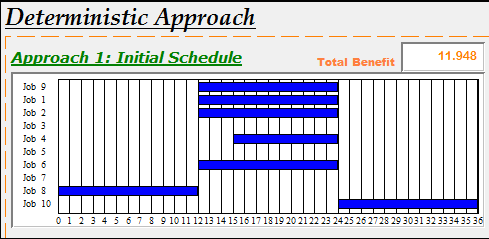
\includegraphics[width=4.5cm,height=2cm]{W14Gamma099.png}}
\setlength\alignwidth{\wd0}
\setlength\alignheight{\ht0}
\sbox2{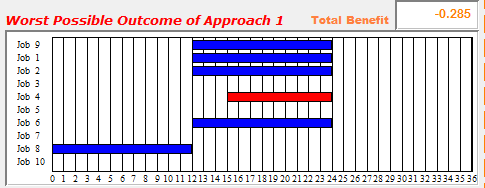
\includegraphics[width=4.5cm,height=2cm]{W14Gamma0992.png}}
\ifdim\wd2>\alignwidth \setlength\alignwidth{\wd2}\fi
\ifdim\ht2>\alignheight \setlength\alignheight{\ht2}\fi
\sbox4{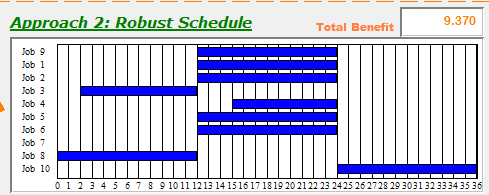
\includegraphics[width=4.5cm,height=2cm]{W14Gamma0993.png}}
\ifdim\ht4>\alignwidth \setlength\alignwidth{\wd4}\fi
\ifdim\ht2>\alignheight \setlength\alignheight{\ht4}\fi
\sbox6{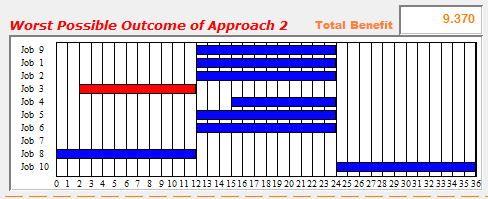
\includegraphics[width=4.5cm,height=2cm]{W14Gamma0994.png}}
\ifdim\ht6>\alignwidth \setlength\alignwidth{\wd6}\fi
\ifdim\ht2>\alignheight \setlength\alignheight{\ht6}\fi

\centering
  \subfloat[Initial Schedule]{\fakeheight{\alignwidth}{\alignheight}{\usebox0}}\hspace{1em}%
  \subfloat[Intial Worst Case]{\fakeheight{\alignwidth}{\alignheight}{\usebox2}}\\[2ex]
  \subfloat[Robust Schedule]{\fakeheight{\alignwidth}{\alignheight}{\usebox4}}\hspace{1em}%
  \subfloat[Robust Worst Case]{\fakeheight{\alignwidth}{\alignheight}{\usebox6}}
\caption{$W=1.4$, $\gamma=0.99$}
%\label{FigData1hp990w1p400}
\end{figure}
\end{frame}

\begin{frame}
\frametitle{Small-size Example}
\begin{figure}[htbp]
\sbox0{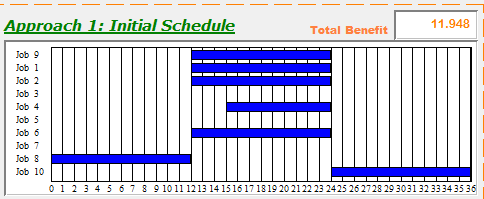
\includegraphics[width=4.5cm,height=2cm]{W25Gamma0991.png}}
\setlength\alignwidth{\wd0}
\setlength\alignheight{\ht0}
\sbox2{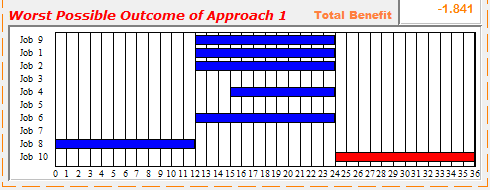
\includegraphics[width=4.5cm,height=2cm]{W25Gamma0992.png}}
\ifdim\wd2>\alignwidth \setlength\alignwidth{\wd2}\fi
\ifdim\ht2>\alignheight \setlength\alignheight{\ht2}\fi
\sbox4{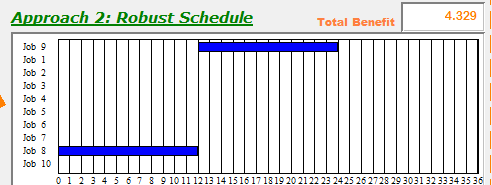
\includegraphics[width=4.5cm,height=2cm]{W25Gamma0993.png}}
\ifdim\ht4>\alignwidth \setlength\alignwidth{\wd4}\fi
\ifdim\ht2>\alignheight \setlength\alignheight{\ht4}\fi
\sbox6{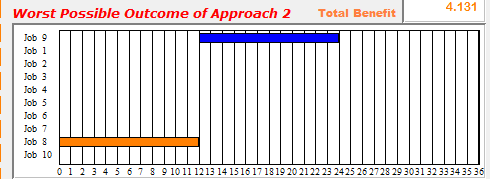
\includegraphics[width=4.5cm,height=2cm]{W25Gamma0994.png}}
\ifdim\ht6>\alignwidth \setlength\alignwidth{\wd6}\fi
\ifdim\ht2>\alignheight \setlength\alignheight{\ht6}\fi

\centering
  \subfloat[Initial Schedule]{\fakeheight{\alignwidth}{\alignheight}{\usebox0}}\hspace{1em}%
  \subfloat[Intial Worst Case]{\fakeheight{\alignwidth}{\alignheight}{\usebox2}}\\[2ex]
  \subfloat[Robust Schedule]{\fakeheight{\alignwidth}{\alignheight}{\usebox4}}\hspace{1em}%
  \subfloat[Robust Worst Case]{\fakeheight{\alignwidth}{\alignheight}{\usebox6}}
\caption{$W=2.5$, $\gamma=0.99$}
\label{FigData1hp990w2p500}
\end{figure}
\end{frame}

\begin{frame}
\frametitle{Small-size Example}
\begin{figure}[htbp]
\sbox0{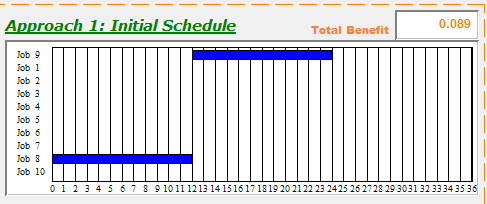
\includegraphics[width=4.5cm,height=2cm]{W25Gamma0951.png}}
\setlength\alignwidth{\wd0}
\setlength\alignheight{\ht0}
\sbox2{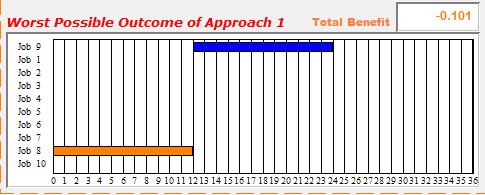
\includegraphics[width=4.5cm,height=2cm]{W25Gamma0952.png}}
\ifdim\wd2>\alignwidth \setlength\alignwidth{\wd2}\fi
\ifdim\ht2>\alignheight \setlength\alignheight{\ht2}\fi
\sbox4{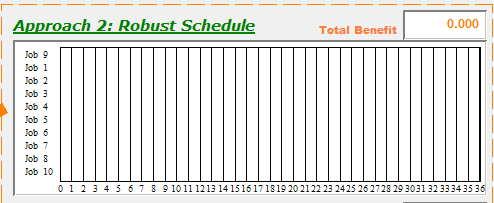
\includegraphics[width=4.5cm,height=2cm]{W25Gamma0953.png}}
\ifdim\ht4>\alignwidth \setlength\alignwidth{\wd4}\fi
\ifdim\ht2>\alignheight \setlength\alignheight{\ht4}\fi
\sbox6{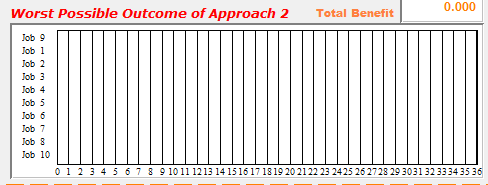
\includegraphics[width=4.5cm,height=2cm]{W25Gamma0954.png}}
\ifdim\ht6>\alignwidth \setlength\alignwidth{\wd6}\fi
\ifdim\ht2>\alignheight \setlength\alignheight{\ht6}\fi

\centering
  \subfloat[Initial Schedule]{\fakeheight{\alignwidth}{\alignheight}{\usebox0}}\hspace{1em}%
  \subfloat[Initial Worst Case]{\fakeheight{\alignwidth}{\alignheight}{\usebox2}}\\[2ex]
  \subfloat[Robust Schedule]{\fakeheight{\alignwidth}{\alignheight}{\usebox4}}\hspace{1em}%
  \subfloat[Robust Worst Case]{\fakeheight{\alignwidth}{\alignheight}{\usebox6}}
\caption{$W=2.5$, $\gamma=0.95$}
%\label{FigData1hp950w2p500}
\end{figure}
\end{frame}

 \begin{frame}
\frametitle{Large-size Example}
$\bullet$ The large-size example contains 77 projects.\\
\bigskip
$\bullet$ We assume the hurdle rate is high and only considers project failure in the worst case scenario.\\
\bigskip
$\bullet$ We approximate the loss incured by the failure on each project in the greedy heuristic.
\end{frame}

\begin{frame}
\frametitle{Large-size Example}
\begin{center}
\includegraphics[scale=0.45] {last.png} 
%\caption{NPV Value VS Bad Luck Budget W}
\end{center}
\end{frame}
		
		\begin{frame}
			\frametitle{Graphical User Interface}
			\begin{center}
				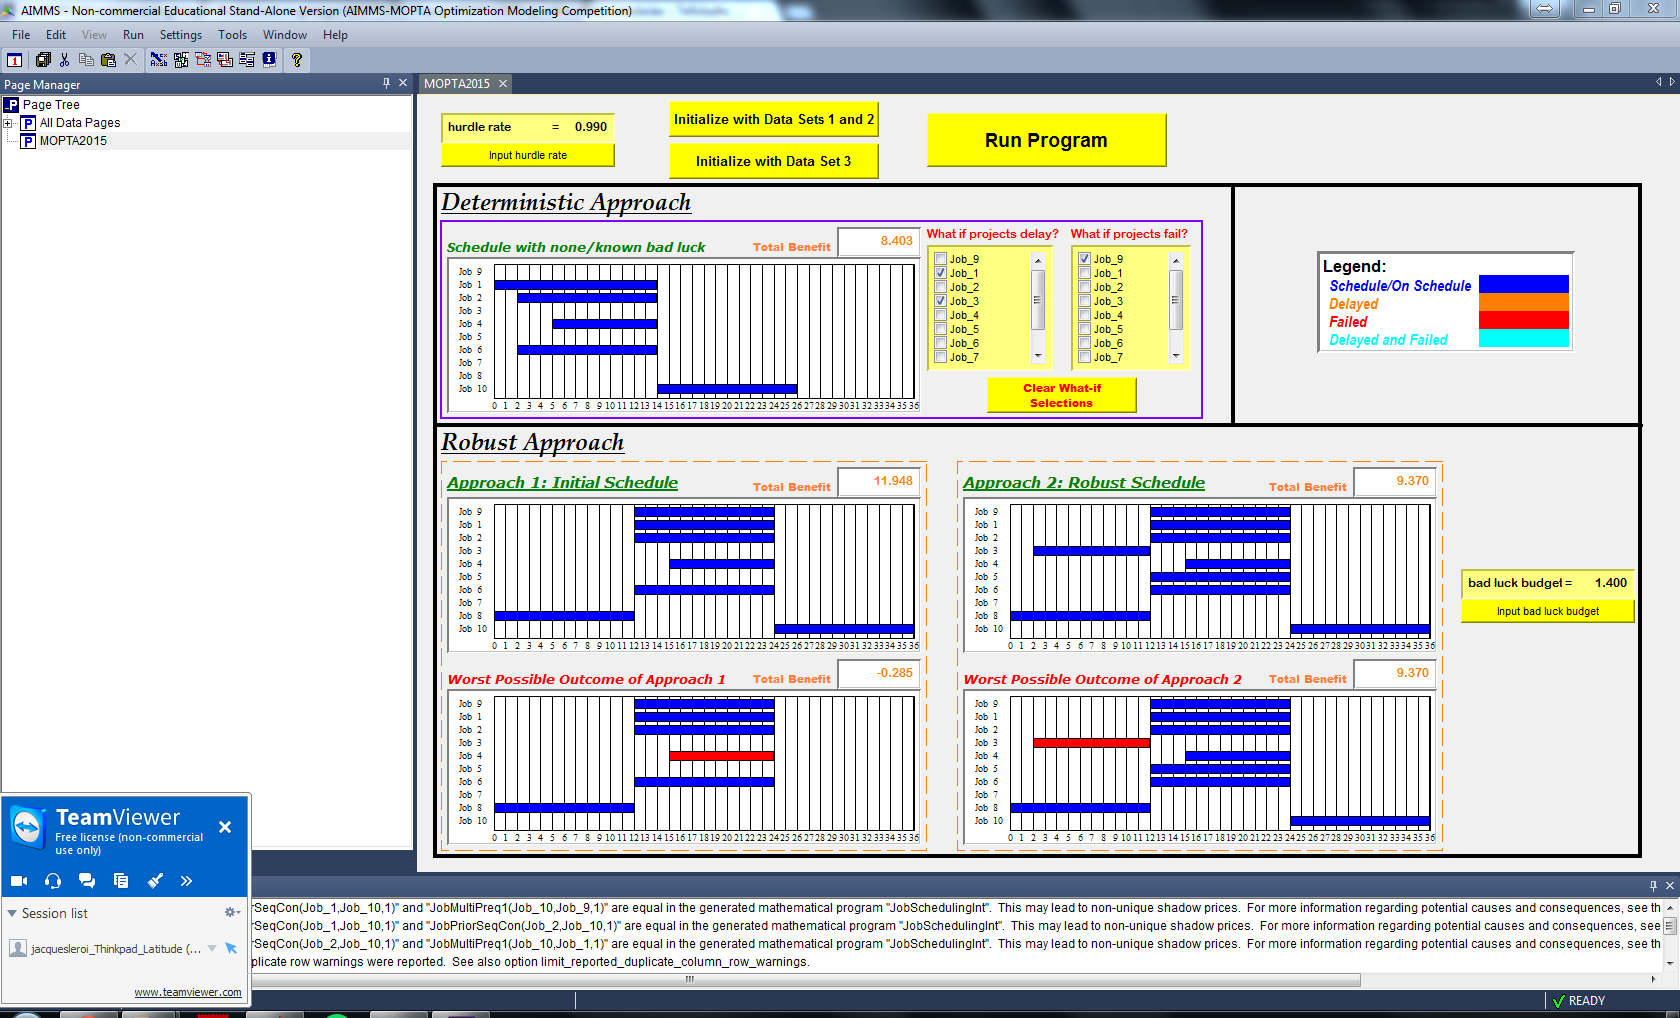
\includegraphics[trim=112mm 40mm 7mm 26mm,clip,scale=0.35]{../MOPTA2015Report/Data1hp990w1p400.png}
			\end{center}
		\end{frame}

	\section*{End}
		\begin{frame}
			\begin{center}
				\Huge Thank you!
			\end{center}
		\end{frame}






\end{document}
